\documentclass[12pt]{article}

\usepackage{fancyhdr}
\usepackage{makeidx}
\usepackage[catalan]{babel}
\usepackage{amsfonts}
\usepackage{amssymb}
\usepackage{amsthm}
\usepackage{amsmath}
\usepackage[all]{xy}
\usepackage[ansinew]{inputenc} %%
\usepackage[dvips]{epsfig}
\usepackage{color}



%\usepackage[spanish]{babel}
%\usepackage{color}% utilitzar color per les letras
%\usepackage{graphics}
%\usepackage{graphicx}
%\usepackage{amssymb}
%\usepackage{amsfonts}%per poder poner les letras de Reales %Complejos etc...
%\usepackage{anysize} % Soporte per el comando \marginsize
%\usepackage[latin1]{inputenc}% permite poner acentos de forma normal

\setlength{\textwidth}{16cm} \setlength{\textheight}{24cm}
\setlength{\oddsidemargin}{-0.3cm} \setlength{\topmargin}{-1.3cm}

%\usepackage{texfonts}
%\marginsize{2cm}{2cm}{2cm}{2cm}
%\newcommand{\ZZ}{\mathbbmss{Z}}
%\usepackage{fancyhdr}
%\renewcommand{\rmdefault}{phv}
%%%%%%%%%%%%%%%%%%%%%%%%%%%%%%%%%%%%%%%%%%%%%%%%%%%%%%%%%%%%%%%%%%%%%%%%
%-- nuevos comandos per facilitar la escritura
\newcommand{\notacio}{\textbf{Notaci{\'o}}\ \ }
\newcommand{\demostracio}{\textbf{Demostraci{\'o}}\ \ }
\newcommand{\propietats}{\textbf{Propietats}\ \ }
\newcommand{\propietat}{\textbf{Propietat}\ \ }
%\newcommand{\exemple}{\textbf{Exemple}\ \ }
\newcommand{\exemples}{\textbf{Exemples}\ \ }
\newcommand{\observacio}{\textbf{Observaci{\'o}}\ \ }
\newcommand{\observacions}{\textbf{Observacions}\ \ }
\newcommand{\solucio}{\textbf{Soluci{\'o}}\ \ }


\newtheorem{definicio}{Definici{\'o}}[subsection]
\newtheorem{teorema}{Teorema}[subsection]
\newtheorem{Teorema}{Teorema}[subsubsection]
\newtheorem{proposicio}{Proposici{\'o}}[subsection]
\newtheorem{lema}{Lema}[subsection]
\newtheorem{corol}{Corol.lari}[subsection]
\newtheorem{exemple}{Exemple}[subsection]
\newtheorem{prob}{Problema}[subsection]


\newcommand{\Z}{\mathbb{Z}}
\newcommand{\R}{\mathbb{R}}
\newcommand{\C}{\mathbb{C}}
\newcommand{\N}{\mathbb{N}}
\newcommand{\U}{\mathcal{U}}
\newcommand{\V}{\mathcal{V}}
\newcommand{\W}{\mathcal{W}}
\newcommand{\sen}{\mathop{\rm sen}\nolimits}

\setcounter{page}{26}

\setcounter{section}{2}

\begin{document}

\parskip =0.3cm
\parindent =0cm
\itemindent=2cm


\vspace{0.4cm}\begin{center}
\section{Diferenciaci{\'o}}
\end{center}


\vspace*{0.7cm}
\subsection{Introducci{\'o} a les derivades parcials}

Considerarem primer una funci{\'o} de dues variables $\ f:\
D\subset \R^{2} \longrightarrow \R\,,$ on $D$ {\'e}s un obert
i $(a,b) \in D$. Si fixam $\ y=b\ $ podem consideram la funci{\'o}

\[
g(x)= f(x,b).
\]

Si  existeix $\ g'(a)$ llavors direm que {\'e}s la \textbf{derivada parcial de $f$
respecte de la variable $x$ en el punt $(a,b)\,.$} Ho denotam per
$f_{x}(a,b)$. D'on

\[
f_{x}(a,b) = g'(a) = \lim_{h\to 0} \frac{g(a+h)-g(a)}{h} =
\lim_{h\to 0} \frac{f(a+h,b)-f(a,b)}{h}
\]

i per tant

\[
f_{x}(a,b) = \lim_{h\to 0} \frac{f(a+h,b)-f(a,b)}{h}
\]

An{\`a}logament, si fixam $\ x=a\ $  podem considerar la funci{\'o}

\[
l(y)=f(a,y),
\]

i si existeix $l'(b)$ li direm \textbf{derivada parcial de $f$
respecte de la variable $y$ en el punt $(a,b)\,,$} i ho
denotarem per $f_{y}(a,b)$. Igualment tenim que

\[
f_{y}(a,b)=l'(b)=\lim_{h\to 0} \frac{l(b+h)-l(b)}{h}
=
\lim_{h\to 0} \frac{f(a,b+h)-f(a,b)}{h}
\]

de forma que

\[
f_{y}(a,b)=\lim_{h\to 0} \frac{f(a,b+h)-f(a,b)}{h}
\]

Per tant, calcular la derivada parcial respecte d'una variable
implica prendre les altres variables com constants i derivar respecte a la variable indicada.

\notacio
Per representar les derivades parcials de $f$
utilitzarem les seg{\"u}ents notacions:

\[
f_{x}(a,b)\qquad\frac{\partial f}{\partial x}(a,b)\qquad
D_{1}f(a,b)\qquad D_{x}f(a,b)
\]
\[
f_y(a,b)\qquad \frac{\partial f}{\partial y}(a,b) \qquad D_2 f(a,b)\qquad D_y
f(a,b)
\]

i si $z=f(a,b)$ escriurem

\[
\frac{\partial f}{\partial x}(a,b)\qquad \frac{\partial z}{\partial
x}(a,b)\qquad z_{x}(a,b)
\]
\[
\frac{\partial f}{\partial y}(a,b)\qquad\frac{\partial y}{\partial
x}(a,b)\qquad z_{y}(a,b)
\]


\vspace{0.4cm}
\begin{exemple}
Si $f(x,y)=x^{3}+x^{2}y^{3}-2y^{2}$; calculau $f_{x}(x,y)\,, \ \ f_{y}(x,y)$ i avaluar-les en el punt $(2,1)$.
\end{exemple}

\solucio

\[
\vspace{0.4cm}
\begin{array}{lcl}
f_{x}(x,y)=3x^{2}+2xy^{3} & \qquad & f_{x}(2,1) = 3 \cdot 2^{2}+2
\cdot 2 \cdot 1^{3} = 16 \\
&\\
 f_{y}(x,y)=3x^{2}y^{2}-4y & \qquad &
f_{y}(2,1) = 3 \cdot 2^{2} \cdot 1^{2} - 4 \cdot 1 = 8
\end{array}
\]

\vspace{0.5cm}

Per veure el significat geom{\`e}tric associat a les derivades parcials d'una
funci{\'o} de dues variables reals recordem que, l'equaci{\'o}
$z=f(x,y)$, representa una superf{\'\i}cie $S$ en $R^{3}\,.$

A partir del significat geom{\`e}tric de la derivada d'una funci{\'o} real
de variable real, tenim que (veure figura \ref{dfdv1}):

\vspace{-0.5cm}
\begin{figure}[h!]
\begin{center}
\input{pagina3.pstex_t}
\end{center}\caption{Significat geom{\`e}tric de les derivades parcials d'una funci{\'o} de dues variables.}\label{dfdv1}
\end{figure}

\begin{itemize}
\item El pla $y=b$ (que {\'e}s paral.lel al pla $xz$) talla a $S$ en una corba $C_{1}$ de tal  manera que   $g'(a)=f_{x}(a,b)$ {\'e}s la pendent de la recta
tangent $T_{1}$ a la corba $C_{1}$ en el punt $(a,b,f(a,b))$.
\item El pla $x=a$ (que {\'e}s paral.lel al pla $yz$) talla a $S$ en una corba $C_{2}$ de tal  manera que   $l'(b)=f_{y}(a,b)$ {\'e}s la pendent de la recta
tangent $T_{2}$ a la corba $C_{2}$ en el punt $(a,b,f(a,b))$.
\end{itemize}

\vspace{0.4cm}
\observacio Els vectors directors de les rectes $T_{1}$ i $T_{2}$ s{\'o}n perpendiculars (ja que  els plans que els generen
s{\'o}n perpendiculars entre s{\'\i}). Aquests vectors juntament amb el
punt $(a, b, f(a,b))$  generen un pla, del que m{\'e}s endavant
parlarem anomenat pla tangent.



\vspace{0.4cm}
\begin{exemple}
Si $f(x,y)=4-x^{2}-2 y^{2}$, calculau $f_{x}(1,1)$ i $f_{y}(1,1)$.
\end{exemple}

\solucio

Tenim que
\[
\vspace{0.4cm}\begin{array}{lcl}
f_{x}(x,y)=-2x, & \quad & f_{x}(1,1) = -2 \\ f_{y}(x,y)=-4y, &
\quad & f_{y}(1,1) = -4
\end{array}
\]

%El graf de $f$ {\'e}s el paraboloide $\ z=4-x^{2}-2y^{2}\ $ i el pla
%vertical $\ y=1\ $ el talla en la par{\`a}bola $\ z=2-x^{2}\,,\ \ y=1$ ({\'e}s a
%dir $\ (x,1,2-x^{2})\,\;  x \in \R)\,.$ El pendent d'aquesta
%par{\`a}bola en el punt $(1,1,1)$ ve donat per
% $\ f_{x}(1,1) = -2\,.$
%De manera similar el pla $\ x=1\ $ interseca al paraboloide en la
%par{\`a}bola $\ z=3-2y^{2}\,,\ \ x=1$ ({\'e}s a dir $\ (1,y,3-2y^{2})\,\; i \in
%\R\ $) i el pendent de la recta tangent a la corba en el punt
%$(1,1,1)$ {\'e}s
%$\ f_{y}(x,y)=-4\,.$


\vspace{0.4cm}
\begin{exemple}
Sigui $\ f(x,y)=\sin \left(\displaystyle\frac{x}{1+y} \right)\,,$ calculau
$\ \displaystyle\frac{\partial f}{\partial x}\ $ i $\ \displaystyle\frac{\partial f}{\partial y}\,.$
\end{exemple}

\solucio
\[
\frac{\partial f}{\partial x}(x,y)=\cos\left(\frac{x}{1+y} \right)
\cdot \frac{1}{1+y}, \quad\quad \frac{\partial f}{\partial
y}(x,y)=\cos\left(\frac{x}{1+y} \right) \cdot \frac{-x}{(1+y)^{2}}.
\]

\vspace{0.4cm}
Donarem ara la definici{\'o} general de derivada parcial per a una funci{\'o} de $n$ variables.

\vspace{0.4cm}
\begin{definicio}
Sigui $\ f:D\subset\R^n\, \longrightarrow\R\,,$ amb  $D$ obert. Sigui
el punt $a\in D$ i consideram el vector unitari $\ u_k =(0,\ldots,  1,\ldots ,0)\,.$
Definim la \textbf{derivada parcial de $f$ respecte de la variable $x_k$ en el punt $a=(a_1,\ldots,a_n)$} i ho denotarem per $f_{x_k}(a)\ $ com

$$
f_{x_k}(a)=\lim_{h\to 0} \frac{f(a+h\, u_k)-f(a)}{h}
$$
\end{definicio}

\vspace{0.4cm}
\observacio
Recordem que en funcions d'una variable real, la derivabilitat en un punt implica la
continu{\"\i}tat en aquest punt. En canvi en el seg{\"u}ent exemple veurem que l'exist{\`e}ncia de derivades
parcials en un punt no implica que la funci{\'o} sigui continua en aquest punt.

\vspace{0.4cm}\begin{exemple}
Sigui $f(x,y)=  \begin{cases}
                       \frac{xy}{x^{2}+3y^{2} }&
\text{si} \,\, (x,y) \neq (0,0)
                        \\
                       0                      &
\text{si} \,\, (x,y) = (0,0)
                    \end{cases}$.
Estudiau la continu{\"\i}tat de $f$ en $(0,0)$ i l'exist{\`e}ncia de
$\frac{\partial f}{\partial x}(0,0)$ i $\frac{\partial f}{\partial
y}(0,0)$.
\end{exemple}

\solucio
Estudiem primer les derivades parcials.
\vspace{0.4cm}
\begin{equation*}
\vspace{0.4cm}\begin{split}
\frac{\partial f}{\partial x}(0,0) & = \lim_{h\to 0}
\frac{f(h,0)-f(0,0)}{h} = \lim_{h\to 0} \frac{0-0}{h} = 0 \\
\frac{\partial f}{\partial y}(0,0) & = \lim_{h\to 0}
\frac{f(0,h)-f(0,0)}{h} = \lim_{h\to 0} \frac{0-0}{h} = 0
\end{split}
\end{equation*}

Ara b{\'e}, $f$ no {\'e}s continua en $(0,0)$ ja que el l{\'\i}mit
\vspace{0.4cm}\begin{equation*}
\lim_{(x,y)\to 0\atop y=mx} f(x,y)=\lim_{x\to 0}
f(x,mx)=\lim_{x\to 0}
\frac{xmx}{x^{2}+3m^{2}x^{2}}=\frac{m}{1+3m^{2}}
\end{equation*}
 dep{\`e}n de $m$ aleshores no existeix el l{\'\i}mit. En definitiva, $f$ no {\'e}s cont{\'\i}nua en $(0,0)$.


Aquest exemple mostra que el concepte de derivada
parcial no generalitza el concepte de derivada d'una
funci{\'o} real de variable real, ara b{\'e} {\'e}s una eina molt
{\'u}til en el estudi de les funcions de diverses variables.


\subsection{Derivades direccionals}

Presentarem ara el concepte de derivada direccional, que t{\'e} com a casos particulars les derivades parcials.

\vspace{0.4cm}
\begin{definicio}
Sigui $f: D\subset\R^n\, \longrightarrow\R\,,\ D$ obert. Sigui
$a\in D$ i el vector $u\in\R^n$ amb $\| u\| =1$.
Direm \textbf{derivada direccional de $f$ en $a$ en la direcci{\'o}
del vector $u$}, i ho denotarem per $D_u f(a)$, al
l{\'\i}mit, si existeix,
\[
D_u f(a) =\lim_{h\to 0}\frac{f(a+h\, u)-f(a)}{h}
\]
\end{definicio}

\observacio Si $f\, :\, D\subset\R^2\, \longrightarrow\R$, $D$ obert i $a=(x_0,y_0)$, $u=(a,b)$ amb $\| u\| =1$ llavors

\[
D_u f((x_0,y_0))=\lim_{h\to 0} \frac{f(x_0+a\,h,y_0+b\,h)-f(x_0,y_0)}{h}
\]

Si consideram $\ u=\overrightarrow{i}=(1,0)\ $ {\'o} $\ u=
\overrightarrow{j}=(0,1)\ $ llavors

\[
D_{\overrightarrow{i}}f(a)=D_1f(a)=\frac{\partial f}{\partial
x}(a),\qquad\qquad D_{\overrightarrow{j}}f(a)=D_2f(a)=\frac{\partial f}{\partial
y}(a).
\]
%Si  $f\, :\, D\subset\R^3\, \longrightarrow\R$, $D$ obert i $a\in D$ si consideram els vectors unitaris $\bigvee
%\overrightarrow{i}=(1,0,0)$, $ \overrightarrow{j}=(0,1,0)$ i $
%\overrightarrow{k}=(0,0,1)$ tenim que
%\[
%D_{\overrightarrow{i}}f(a)=D_1f(a)=\frac{\partial f}{\partial
%x}(a),\, D_{\overrightarrow{j}}f(a)=D_2f(a)=\frac{\partial f}{\partial
%y}(a),\, D_{\overrightarrow{k}}f(a)=D_3f(a)=\frac{\partial f}{\partial
%z}(a).
%\]

En general si $f\, :\, D\subset\R^n\, \longrightarrow\R$, $D$ obert. Sigui
el punt $a\in D$ i consideram el vector unitari $u_k =
(0,\ldots,  1,\ldots ,0)$ es t{\'e} que
\[
D_{u_k}f(a)=\frac{\partial f}{\partial
x_k}(a)\,.
\]


\vspace{0.4cm}
\begin{exemple}\label{exempderdir}
Considerem la funci{\'o} $f(x,y)=2x^2+3y^2$. Calculau la derivada direccional de la funci{\'o} $f$ en el punt $(1,0)$ i en la direcci{\'o} que forma amb l'eix $x$ un angle de $\frac{2\pi}{3}$ radians.
\end{exemple}

\solucio
La direcci{\'o} ve donada pel vector
\[
u=\left(\cos \frac{2\pi}{3},\sin \frac{2\pi}{3}\right )=\left(-\frac{1}{2},\frac{\sqrt{3}}{2}\right)\,\;
\mbox{on}\ \ \| u\| =1.
\]
Aix{\'\i}, utilitzant la definici{\'o} tenim que
\vspace{0.4cm}\begin{align*}
  D_uf(a) = & \lim_{h\to 0}\frac{f(a+h\, u)-f(a)}{h}  \\
   = & \lim_{h\to 0}\frac{f((1,0) +h
   (-\frac{1}{2},\frac{\sqrt{3}}{2}))-f(1,0)}{h}\\
   = &  \lim_{h\to 0} \frac{f(1-\frac{h}{2},h
   \frac{\sqrt{3}}{2})-f(1,0)}{h} \\
   = &  \lim_{h\to 0} \frac{2 (1-\frac{h}{2} )^2 + 3 (h \frac{\sqrt{3}}{2} )^2 -2 }{h}
  =  \lim_{h\to 0} \frac{\frac{11}{4}h^2 - 2h}{h}=-2
\end{align*}
per tant
\[
D_uf(1,0)=-2.
\]

\vspace{0.3cm}
M{\'e}s endavant presentarem una manera de calcular les derivades direccionals,
sense tenir que fer el l{\'\i}mit donat en la definici{\'o}.

\subsection{Diferenciabilitat. Diferencial}

En la seg{\"u}ent definici{\'o} generalitzarem el concepte de diferenciabilitat a
funcions de diverses variables.

\vspace{0.4cm}
\begin{definicio}
Sigui una funci{\'o} vectorial de variable vectorial,
$f:D \subseteq \R^{n} \longrightarrow \R^m\,,\ D$
obert i $a \in D $, direm que \textbf{$f$ {\'e}s diferenciable en
$a \in D $} si existeix una aplicaci{\'o} lineal $\ L_a: \R^{n}
\longrightarrow \R^m\ $ verificant que

\[
\lim_{h \to 0} \frac{f(a+h) - f(a) - L_a(h) }{\| h \|} = 0
\]
\end{definicio}


\vspace{0.4cm}
\begin{definicio}
A l'aplicaci{\'o} lineal $\ L_a: \R^{n} \longrightarrow \R^m\ $ se li
diu \textbf{diferencial de $f$ en $a$} i es denota
per $Df(a)$ o $df(a)$.
\end{definicio}

\vspace{0.4cm}
\begin{definicio}
Sigui
$\ f:D \subseteq \R^{n} \longrightarrow \R^m\,,\ D$
obert, direm que \textbf{$f$ {\'e}s diferenciable en $D$}  si {\'e}s diferenciable en tots els punts de $D$.
\end{definicio}


\vspace{0.4cm}
\begin{definicio}
La matriu associada a l'aplicaci{\'o} lineal $Df(a)$ respecte de les bases can{\`o}niques s'anomena \textbf{matriu jacobiana} de $f$  en el punt $a$ i ho denotam per $\ Jf(a)$.
\end{definicio}

\vspace{0.4cm}
\begin{teorema}
Si $f:D \subseteq\R^n \longrightarrow \R^m$ {\'e}s diferenciable en
$a$, llavors la matriu jacobiana de $f$ en $a$ {\'e}s:


$$ Jf(a) = \left( \vspace{0.4cm}\begin{array} {cccc}
\displaystyle\frac{\partial f_1}{\partial x_1}(a) & \displaystyle\frac{\partial f_1}{\partial x_2}(a) &
\ldots & \displaystyle\frac{\partial f_1}{\partial x_n}(a)\\
\\
\displaystyle\frac{\partial f_2}{\partial x_1}(a) & \displaystyle\frac{\partial f_2}{\partial x_2}(a) &
\ldots & \displaystyle\frac{\partial f_2}{\partial x_n}(a)\\
\vdots & \vdots & \ddots & \vdots \\
\displaystyle\frac{\partial f_m}{\partial x_1}(a) & \displaystyle\frac{\partial f_m}{\partial x_2}(a) &
\ldots & \displaystyle\frac{\partial f_m}{\partial x_n}(a)\\
                   \end{array} \right) $$
\end{teorema}

\vspace{0.4cm}
\begin{exemple}
Considerem la funci{\'o}
\begin{align*}
    f\, :\, \R^2 & \longrightarrow  \R^3 \\
    (x,y) & \mapsto \left( 1+e^x,\sin(xy),\frac{x}{y} \right) \\
\end{align*}
Calculau la matriu jacobiana de $f$ en el punt $(0,2)$.
\end{exemple}

\solucio Calculem les derivades parcials de cada una de les funcions components.
\vspace{0.4cm}\begin{align*}
   f_1\,  : \, \R^2 & \longrightarrow  \R \quad
  & f_2\, : \, \R^2 & \longrightarrow  \R \quad
  & f_3\, : \, D & \longrightarrow  \R \\
  (x,y) &  \mapsto  1+e^x
  & (x,y) & \mapsto  \sin(xy)
  &(x,y) & \mapsto \frac{x}{y}
\end{align*}
\begin{align*}
& \frac{\partial f_1}{\partial x}(x,y)   = e^x \quad  &
\frac{\partial f_2}{\partial x}(x,y)   & =
  y\cos (xy) \quad    & \frac{\partial f_3}{\partial
x}(x,y)  &  = \frac{1}{y}    \\ & \frac{\partial f_1}{\partial
y}(x,y)   =
 0 \quad  & \frac{\partial f_2}{\partial
y}(x,y)  & =
  x\cos (xy) \quad   & \frac{\partial f_3}{\partial
y}(x,y)  & =
 -\frac{x}{y^2}
  \end{align*}

Tenim que la matriu jacobiana en un punt qualsevol del domini de $f$ val:

\begin{equation*}
Jf(x,y) =  \left( \vspace{0.4cm}\begin{array} {cc}
   e^x & 0 \\
   \\
   y \cos(xy) & x \cos(xy) \\
   \\
   \displaystyle\frac{1}{y} & -\displaystyle\frac{x}{y^2} \\
\end{array} \right)
\end{equation*}

Per tant

\vspace{0.4cm}\begin{equation*}
Jf(0,2) = \left( \vspace{0.4cm}\begin{array} {cc}
   e^0 & 0\\
   2 \cos 0 & 0 \cos 0 \\
   \frac{1}{2} & -\frac{0}{2^2} \\
\end{array} \right) = \left( \vspace{0.4cm}\begin{array} {cc}
   1 & 0 \\
   2 & 0 \\
   \frac{1}{2} & 0 \\
\end{array}\right)
\end{equation*}


%\vspace{0.4cm}
%\begin{exemple}
%Sigui $U$ un obert de $\R^m$ i $f:U  \subseteq \R^n
%\longrightarrow \R^m$. llavors:
%\begin{itemize}
%\item[a)] Si $f$ {\'e}s una funci{\'o} constant, llavors $Df(a)=0 \,,\quad \forall a \in U$.
%\item[b)] Si
%$f$ {\'e}s una aplicaci{\'o} lineal, llavors $Df(a)=f \,,\quad \forall a \in U$.
%\end{itemize}
%\end{exemple}
%
%\solucio
%
%a) $\displaystyle{\lim\limits_{h\to 0} \frac{ f(a+h) - f(a) - 0
%}{\left| \left| h \right| \right|} = \lim\limits_{h \to 0}
%\frac{ c - c - 0}{\left| \left| h
%\right| \right|}= \lim\limits_{h \to 0} \frac{0}{\left| \left| h \right|
%\right|} = 0}$
%
%\vspace{0.4cm}
%b) $\displaystyle{\lim\limits_{h\to 0} \frac{f(a+h) - f(a) - f(h)
%}{\left| \left| h \right| \right|} = \lim\limits_{h \to 0}
%\frac{ f(a+h) - f(a+h)}{\left| \left|
%h \right| \right|}= \lim\limits_{h \to 0} \frac{ 0}{\left| \left| h \right| \right|} = 0}$

\vspace{0.4cm}
Donarem ara una s{\`e}rie de propietats relacionades amb les funcions diferenciables.

\vspace{0.4cm}
\begin{teorema}
Si $f:D \subseteq\R^n \longrightarrow \R^m$ {\'e}s diferenciable en
$a$, llavors $f$ {\'e}s cont{\'\i}nua en $a$.
\end{teorema}


%\vspace{0.4cm}
%\begin{teorema}\label{teorema2}
%Si $f:D \subseteq \R^n \longrightarrow \R$ {\'e}s diferenciable en
%$a\in D$, llavors existeixen totes les derivades direccionals de $f$ en $a$. A m{\'e}s
%
%$$
%D_u f(a) =Df(a)(u)=Jf(a)\cdot u
%$$
%
%on aquest darrer producte, correspon al producte matricial.
%\end{teorema}


%\vspace{0.4cm}
%\observacio Existeixen funcions que tenen totes les derivades direccionals en un punt, per{\`o} no s{\'o}n diferenciables en aquest punt.

\vspace{0.4cm}
\begin{teorema}
Si $\ f:D \subseteq\R^n \longrightarrow \R^m\ $ verifica que en un entorn de $a$, existeixen totes les derivades parcials i s{\'o}n funcions cont{\'\i}nues,  llavors $f$  {\'e}s diferenciable en $a$.
\end{teorema}




\vspace{0.4cm}
\subsection{Gradient. Pla tangent}

\vspace{0.4cm}
\begin{definicio}
Sigui $f:D\subset\R^n\, \longrightarrow\R$, $D$ obert i el punt $a\in D$, suposem que existeixen totes les derivades
parcials de $f$ en el punt $a$. Definim el \textbf{vector
gradient de $f$ en $a$} com el vector
\[
\nabla f(a)=\left(\frac{\partial f}{\partial x_1}(a),\frac{\partial f}{\partial x_2}(a), \ldots , \frac{\partial f}{\partial x_n}(a)\right)
\]
\end{definicio}

\vspace{0.4cm}
\observacio Es pot demostrar que el vector gradient ens dona la direcci{\'o} en la qual $f$ creix m{\'e}s r{\`a}pidament.

%\vspace{0.4cm}
%La relaci{\'o} existent entre les derivades direccionals i el
%vector gradient ve donada pel seg{\"u}ent resultat que {\'e}s una conseq{\"u}{\`e}ncia immediata del teorema  \ref{teorema2}.

\vspace{0.4cm}
\begin{corol}\label{cor1}
Siguin $f:D\subset\R^n\, \longrightarrow\R\,,\ D$ obert i $a\in D$. Suposem que $f$ {\'e}s diferenciable en $a$. Llavors la derivada direccional de $f$
segons qualsevol vector unitari $u$  es pot calcular com el seg{\"u}ent producte escalar
\[
D_uf(a)  = \nabla f(a)\cdot u
\]
\end{corol}

Aplicarem aquest resultat a repetir el c{\`a}lcul fet a l'exemple \ref{exempderdir}.

\vspace{0.4cm}
\begin{exemple}
Considerem la funci{\'o} $f(x,y)=2x^2+3y^2$. Calculau la derivada direccional de la funci{\'o} $f$ en el punt $(1,0)$ i en la direcci{\'o} que forma amb l'eix $x$ un angle de $\frac{2\pi}{3}$ radians.
\end{exemple}

\solucio Calculam primer les derivades parcials de $f$:

$$
\frac{\partial f}{\partial x}(x,y)=4 x\qquad\qquad \frac{\partial f}{\partial y}(x,y)=6 y
$$
$$
\frac{\partial f}{\partial x}(1,0)=4 \qquad\qquad \frac{\partial f}{\partial y}(1,0)=0
$$

Per tant el gradient en aquest punt val: $\ \nabla f(1,0)=\left(\frac{\partial f}{\partial x}(1,0),\frac{\partial f}{\partial y}(1,0)\right)=(4,0)\,.$

La direcci{\'o} ve donada pel vector

\[
u=\left(\cos \frac{2\pi}{3},\sin \frac{2\pi}{3} \right)=\left(-\frac{1}{2},\frac{\sqrt{3}}{2}\right)\,\;
\mbox{on}\ \ \| u\| =1.
\]

Aix{\'\i}, utilitzant el resultat del corol.lari anterior
$$
D_uf(1,0)=\nabla f(1,0)\cdot u=(4,0)\cdot \left(-\frac{1}{2},\frac{\sqrt{3}}{2}\right)=-2
$$


\vspace{0.4cm}
\begin{exemple}
Calculau la derivada direccional $\ D_uf(1,2)\ $ si $\ f(x,y)=x^3 -3xy +
4y^2\ $ i $\ u\ $ {\'e}s el vector unitari donat per l'angle $\theta
=\frac{\pi}{6}\,.$
\end{exemple}

\solucio
El vector $u$ ve donat per
\[
u=\left(\cos \frac{\pi}{6},\sin \frac{\pi}{6}\right)= \left(\frac{\sqrt{3}}{2}
,\frac{1}{2}\right).
\]

Calculam ara les derivades parcials de $f$:

$$
\frac{\partial f}{\partial x}(x,y)=3 x^2-3y\qquad\qquad \frac{\partial f}{\partial y}(x,y)=-3x+8 y
$$
$$
\frac{\partial f}{\partial x}(1,2)=-3 \qquad\qquad \frac{\partial f}{\partial y}(1,2)=13
$$

Per tant el gradient en aquest punt val: $\ \nabla f(1,2)=\left(\frac{\partial f}{\partial x}(1,2),\frac{\partial f}{\partial y}(1,2)\right)=(-3,13)\,.$

per tant
\[
D_uf(1,2)=(-3,13)\cdot\left(\frac{\sqrt{3}}{2}
,\frac{1}{2}\right)= \frac{13-3\sqrt{3}}{2}
\]

%\vspace{0.4cm}
%\begin{exemple}
%Si $f(x,y,z)=x\sin (yz)$ es demana:
%\vspace{0.4cm}\begin{itemize}
%  \item[a)] Calculau el gradient de $f$ en qualsevol punt
%  $(x,y,z)$.
%  \item[b)] Trobau la derivada direccional de $f$ en el punt $(1,3,0)$
%  i en la direcci{\'o} del vector $v= i + 2  j- k$.
%\end{itemize}
%\end{exemple}
%
%\solucio
%a)
%\vspace{-0.9cm}
%\begin{align*}
%\nabla f(x,y,z)& =\left( \frac{\partial f}{\partial x}(x,y,z),\frac{\partial f}{\partial y}(x,y,z),\frac{\partial f}{\partial z}(x,y,z) \right) \\ &
%\\ &
% = (\sin (yz),xz\cos (yz),xy\cos
%(yz)).
%  \end{align*}
%b) En $(1,3,0)$ es t{\'e} que
%  \[
%\nabla f(1,3,0) = (0,0,3).
%  \]
%  Per calcular $D_u f (1,3,0)$ tenim que prendre el vector
%  unitari $u$ en la direcci{\'o} de $v= i + 2  j- k$. Com $\ \| v\| =
%  \sqrt{6}\ $ tenim que
%$$u= \frac{v}{\| v\|} = \frac{1}{\sqrt{6}}
%  \,i+ \frac{2}{\sqrt{6}} \,j -
%  \frac{1}{\sqrt{6}}\, k$$
%
% Aix{\'\i}
%  \[
%D_u f (1,3,0) = \nabla f(1,3,0)\cdot u  = -\frac{\sqrt{6}}{2}
%  \]


\vspace{0.4cm}
\begin{definicio}
Sigui  $\ f:D  \subseteq \R^2\longrightarrow \R\,, \ D$  obert. Sabem que l'equaci{\'o} $z=f(x,y)$ representa una superf{\'\i}cie $S$. Definim  \textbf{el pla tangent} de $S$ en el punt $(x_0,y_0,f(x_0,y_0))\in S$ com:
$$z=f(x_0,y_0)+\frac{\partial f}{\partial x}(x-x_0)+\frac{\partial f}{\partial y}(y-y_0)$$
\end{definicio}


\vspace{0.4cm}
\begin{figure}[h]
\begin{center}
\input{pagina14.pstex_t}
\end{center}\caption{Pla tangent a $S$ en el punt $\ (x_0,y_0,(f(x_0,y_0))$.}\label{dfdv3}
\end{figure}

\vspace{0.4cm}
\begin{exemple}
Trobau el pla tangent a la superf{\'\i}cie $\ z=2x^{2}+y^{2}\ $ en el punt $(1,1,3)$.
\end{exemple}

\solucio
Sigui $f(x,y)=2x^{2}+y^{2}$ i observau que $f(1,1)=3$. Les derivades parcials en el punt $(1,1)$ s{\'o}n
\begin{align*}
\frac{\partial f}{\partial x}(x,y) & =4x & \frac{\partial
f}{\partial y}(x,y) & =2y \\ \frac{\partial f}{\partial x}(1,1) &
=4 & \frac{\partial f}{\partial y}(1,1) & =2
\end{align*}

aix{\'\i}, l'equaci{\'o} del pla tangent {\'e}s:
\vspace{0.4cm}\begin{equation*}
z = 3+4(x-1)+2(y-1) \,\, \Longrightarrow  \, \, z=3+4x-4+2y-2 \,\,
\Longrightarrow  \, \, 4x+2y-z-3=0
\end{equation*}

\subsection{Regla de la cadena}
Com ja sabem, la composici{\'o} de funcions est{\`a} present de manera majorit{\`a}ria dins el conjunt de les funcions, d'aqu{\'\i} l'import{\`a}ncia del seg{\"u}ent resultat.

\vspace{0.4cm}
\begin{teorema} (Regla de la cadena)

Sigui  $f:U \longrightarrow
\R^m\,,\ U$ obert de $\R^n$, $f$ diferenciable en $\ a \in U\,.$ Sigui $\ g:V
\longrightarrow \R^p\ $ on $\ V\ $ {\'e}s un obert de $\ \R^m\,, $ tal que $\ f(U)
\subset V\ $ i $\ g$ diferenciable en $\ f(a)$. Llavors $g\circ
f:U \longrightarrow \R^p$ {\'e}s diferenciable en $a\ $ i es verifica que
\[
J(g\circ f)(a) = Jg(f(a)) \cdot Jf(a)
\]
\end{teorema}


\vspace{0.4cm}
\begin{exemple}
Si $\ z=x^2y+3xy^4\,,$ on $\ x=e^t\,,\ y=\sin t$, calculau
$\displaystyle\frac{dz}{dt}$
\end{exemple}

\solucio
Si consideram les funcions: $\ f:\R\longrightarrow \R^2\,,\quad g:\R^2\longrightarrow \R\ $ definides per $\ f(t)=(e^t,\sin t)\,, \quad g(x,y)=x^2y+3xy^4,$ aleshores la nostra funci{\'o} $z$ {\'e}s $\ h:\R\longrightarrow \R\ $ definida per $\ h=g\circ f\,.$ Ja que les funcions $f$ i $g$ s{\'o}n diferenciables en tot el seu domini (tenen totes les derivades parcials i s{\'o}n cont{\'\i}nues), llavors  $h$ {\'e}s diferenciable.

Calculem les seves matrius jacobianes:
\begin{equation*}
Jf=\left(\begin{array} {c}
  \displaystyle\frac{d\,f_1}{d\, t} \\
   \\
   \displaystyle\frac{d\, f_2}{d\, t} \\
   \end{array} \right)=\left(\begin{array} {c}
   e^t \\
   \\
   \cos t \\
   \end{array} \right)
   \qquad\qquad Jg=\left(\begin{array} {cc}
   \displaystyle\frac{\partial g}{\partial x} & \displaystyle\frac{\partial g}{\partial y}
\end{array} \right)=\left(\begin{array} {cc}
 2xy+3y^4  & x^2+12xy^3
\end{array} \right)
\end{equation*}


\begin{equation*}
Jh=Jg\cdot Jf = (
(2xy+3y^4)e^t+(x^2+12xy^3)\cos t)= ( (2e^t\sin
t+3\sin^4t)e^t+(e^{2t}+12\,e^t \sin^3t)\cos t)
\end{equation*}

En definitiva, $\ \displaystyle\frac{dz}{dt}(t)=h'(t)=(2e^t\sin
t+3\sin^4t)e^t+(e^{2t}+12\,e^t\sin^3t)\cos t$

\vspace{0.4cm}
Molt sovint es fa el c{\`a}lcul anterior de la seg{\"u}ent manera:
\begin{align*}
\frac{dz}{dt} & = \frac{\partial f}{\partial x} \frac{dx}{dt} +
\frac{\partial f}{\partial y} \frac{dy}{dt} =
(2xy+3y^4)e^t+(x^2+\,12xy^3)\cos t= \\
&\\ & = (2e^t\sin
t+3\sin^4t)e^t+(e^{2t}+12\,e^t\sin^3t)\cos t
\end{align*}

\vspace{0.4cm}
\begin{exemple}
Si $\ z=e^x \sin y\ $ on $\ x=s\, t\,,\ y=s + t$, calculau
$\ \displaystyle\frac{\partial z}{\partial s}\ $ i $\ \displaystyle\frac{\partial z}{\partial t}\,$
\end{exemple}

\solucio
Si consideram les funcions: $\ f:\R^2\longrightarrow \R^2\,,\quad g:\R^2\longrightarrow \R\ $ definides per $\ f(s,t)=(s\,t,s+ t)\,, \quad g(x,y)=e^x \sin y,$ aleshores la nostra funci{\'o} $z$ {\'e}s $\ h:\R^2\longrightarrow \R\ $ definida per $\ h=g\circ f\,.$ Ja que les funcions $f$ i $g$ s{\'o}n diferenciables en tot el seu domini (tenen totes les derivades parcials i s{\'o}n cont{\'\i}nues), llavors  $h$ {\'e}s diferenciable.

Calculem les seves matrius jacobianes:
\begin{equation*}
Jf=\left(\begin{array} {cc}
   \displaystyle\frac{\partial f_1}{\partial s} & \displaystyle\frac{\partial f_1}{\partial t} \\
   &\\
   \displaystyle\frac{\partial f_2}{\partial s} & \displaystyle\frac{\partial f_2}{\partial t} \\
   \end{array} \right)=
   \left(\begin{array} {cc}
   t &  s \\
  &\\
  1 & 1 \\
   \end{array} \right)
   \qquad\qquad Jg=\left(\begin{array} {cc}
  \displaystyle \frac{\partial g}{\partial x} & \displaystyle\frac{\partial g}{\partial y}
\end{array} \right)=\left(\begin{array} {cc}
 e^x \sin y  & e^x \cos y
\end{array} \right)
\end{equation*}

\begin{equation*}
Jh=Jg\cdot Jf = \left(\begin{array} {cc}
 e^x \sin y  & e^x \cos y
\end{array} \right)\left(\begin{array} {cc}
   t & s \\
  &\\
  1 & 1 \\
   \end{array} \right)\\
\end{equation*}

\begin{equation*}
   =\left(\begin{array} {cc}
 t e^x \sin y + e^x
\cos y  & se^x \sin y +  e^x\cos y
\end{array} \right)
\end{equation*}

\begin{equation*}
   =\left(\begin{array} {cc}
 t e^{s t}\sin (s+ t) +  e^{s t} \cos (s+ t)  &
  s e^{s t}\sin (s+t) +  e^{s t} \cos (s+t)
\end{array} \right)
\end{equation*}

\vspace{0.4cm}
Com abans, es pot fer de la seg{\"u}ent manera
\begin{align*}
\frac{\partial z}{\partial s}=\frac{\partial z}{\partial x}
\cdot \frac{\partial x}{\partial s} + \frac{\partial z}{\partial
y} \cdot \frac{\partial y}{\partial s}  & = (e^x \sin y)(t) + (e^x
\cos y)(1) \\
& = t e^{s t}\sin (s+ t) +  e^{s t} \cos (s+ t)
\end{align*}
\vskip -0.8 cm
\vspace{0.4cm}\begin{align*}
\frac{\partial z}{\partial t}=\frac{\partial z}{\partial x}
\cdot \frac{\partial x}{\partial t} + \frac{\partial z}{\partial
y} \cdot \frac{\partial y}{\partial t} & = (e^x \sin y)(s) + (e^x
\cos y)(1) \\
& = s e^{s t}\sin (s+t) +  e^{s t} \cos (s+t)
\end{align*}

%\vspace{0.4cm}
%\begin{exemple}
%Si $\ g(s,t) = f(s^2-t^2, t^2-s^2)\ $ i $\ f\ $ {\'e}s diferenciable,
%comprovau que $\ g\ $ verifica l'equaci{\'o}: $$ t \frac{\partial
%g}{\partial s} + s \frac{\partial g}{\partial t} = 0$$
%\end{exemple}
%
%\solucio
%Si $\ x=s^2-t^2\,,\ \ y=t^2-s^2$; llavors aplicant la regla de la
%cadena:
%
%\[
%\frac{\partial g}{\partial s} = \frac{\partial
%f}{\partial x} \cdot \frac{\partial x}{\partial s} +
%\frac{\partial f}{\partial y} \cdot \frac{\partial y}{\partial s}
%= \frac{\partial f}{\partial x} 2 s + \frac{\partial f}{\partial y}
%(-2 s)
%\]
%\[
%\frac{\partial g}{\partial t} = \frac{\partial f}{\partial x}
%\cdot \frac{\partial x}{\partial t} + \frac{\partial f}{\partial
%y} \cdot \frac{\partial y}{\partial t} = \frac{\partial
%f}{\partial x} (-2 t) + \frac{\partial f}{\partial y} 2 t
%\]
%per tant:
%
%\vspace{0.4cm}
%\begin{align*}
%t \frac{\partial g}{\partial s} + s
%\frac{\partial g}{\partial t} = & t \left( \frac{\partial
%f}{\partial x} 2 s - \frac{\partial f}{\partial y} 2 s \right) +  s
%\left( - \frac{\partial f}{\partial x} 2t - \frac{\partial
%f}{\partial y} 2 t \right) \\
%&\\
% = & 2 t s \frac{\partial f}{\partial x} -
%2ts \frac{\partial f}{\partial y} - 2 t s \frac{\partial f}{\partial
%x} + 2 t s \frac{\partial f}{\partial y} = 0
%\end{align*}
%
%\vspace{0.4cm}
%\begin{exemple}
%Siguin $\ g(x,y)=(x^2+1,y^2)\ $ i $\ f(u,v) = (u+v,u,v^2)\,,$ calculau la
%diferencial de $\ f\circ g\ $ en el punt $\ (1,1)\ $ utilitzant la regla de
%la cadena.
%\end{exemple}
%
%\solucio
%Si observam $f$ i $g$ tenim que  verifiquen les hip{\`o}tesis
%de la regla de la cadena. Aix{\'\i}, i ja que $\ g(1,1) = (2,1)$:
%\[
%D(f\circ g)(1,1) =Df(g(1,1))\circ Dg(1,1)=Df(2,1)\circ Dg(1,1)
%\]
%
%Calcularem la matriu jacobiana corresponent. Per aix{\`o} calculam primer:
%
%\[
%Jf(u,v) = \left(\begin{array} {cc}
% \displaystyle{ \frac{\partial f_1}{\partial u}} &
% \displaystyle{\frac{\partial f_1}{\partial
%  v}} \\
%\\
%  \displaystyle{\frac{\partial f_2}{\partial u}} &
%  \displaystyle{\frac{\partial f_2}{\partial
%  v}} \\
%\\
%  \displaystyle{\frac{\partial f_3}{\partial u}} &
%  \displaystyle{\frac{\partial f_3}{\partial v}}
%\end{array} \right) = \left(\begin{array} {cc}
%  1 & 1 \\
%  1 & 0 \\
%  0 & 2v
%\end{array} \right)
%\]
%
%\[
%Jg(x,y) = \left(\begin{array} {cc}
%  \displaystyle{\frac{\partial g_1}{\partial x}} &
%  \displaystyle{\frac{\partial g_1}{\partial
%  y}} \\
% \\
% \displaystyle{ \frac{\partial g_2}{\partial x}} &
% \displaystyle{\frac{\partial g_2}{\partial y}} \\
% \\
%\end{array} \right) = \left(\begin{array} {cc}
%  2x & 0 \\
%  0 & 2y
%\end{array} \right)
%\]
%
%Per tant,
%
%\[
%J(f\circ
%g){(1,1)}
%=
%Jf(2,1)\cdot Jg(1,1) = \left(\begin{array} {cc}
%  1 & 1 \\
%  1 & 0 \\
%  0 & 2
%\end{array} \right) \left(\begin{array} {cc}
%  2 & 0 \\
%  0 & 2
%\end{array} \right) = \left(\begin{array} {cc}
%  2 & 2 \\
%  2 & 0 \\
%  0 & 4
%\end{array} \right)
%\]

\vspace{0.4cm}

\subsection{Derivades parcials d'ordre superior}

Sigui $f:D \subseteq \R^{2} \longrightarrow \R$ $D$ obert.
Suposem que existeixen les derivades parcials de $f$ en cada
punt de $D,$ llavors, $f_{x}$, $f_{y}$ s{\'o}n funcions de les quals hi ha la possibilitat de calcular les seves derivades parcials
%\[
%\vspace{0.4cm}\begin{array}{lccr}
%\vspace{0.4cm}\begin{diagram}
%\node{}\node{\left(f_x \right)_x} \\ \node{f_x} \arrow{ne,t}{}
%\arrow{se,b}{} \\ \node{}\node{\left(f_x \right)_y}
%\end{diagram}
%& \quad \quad &
%\vspace{0.4cm}\begin{diagram}
%\node{}\node{\left(f_x \right)_x} \\ \node{f_x} \arrow{ne,t}{}
%\arrow{se,b}{} \\ \node{}\node{\left(f_x \right)_y}
%\end{diagram}
%\end{array}
%\]
$(f_{x})_{x}$, $(f_{x})_{y}$, $(f_{y})_{x}$, $(f_{y})_{y}$,
que reben el nom de \textbf{derivades parcials de
segon ordre de $f$} (en el punt considerat).
Utilitzarem la seg{\"u}ent notaci{\'o}:

\begin{equation*}
\begin{split}
(f_{x})_{x} & \qquad f_{xx} \qquad \frac{\partial}{\partial x} \left(
\frac{\partial f}{\partial x} \right) \qquad \frac{\partial^{2}
f}{\partial x^{2}} \qquad D_{11}f \\
&\\
(f_{x})_{y} &  \qquad f_{xy} \qquad \frac{\partial}{\partial y} \left( \frac{\partial
f}{\partial x} \right) \qquad \frac{\partial^{2} f}{\partial y \partial
x} \qquad D_{12} f \\
&\\
(f_{y})_{x} &  \qquad f_{yx} \qquad \frac{\partial}{\partial x} \left( \frac{\partial
f}{\partial y} \right) \qquad \frac{\partial^{2} f}{\partial x \partial
y} \qquad D_{21} f \\
&\\
(f_{y})_{y} &  \qquad f_{yy} \qquad \frac{\partial}{\partial y} \left( \frac{\partial
f}{\partial y} \right) \qquad \frac{\partial^{2} f}{\partial
y^{2}} \qquad D_{22}f
\end{split}
\end{equation*}

\observacio {\'E}s important notar com {\'e}s l'ordre de les variables en les diferents notacions.

De la mateixa manera, cada una d'aquestes derivades parcials de
segon ordre pot admetre derivades parcials,
obtenint les \textbf{derivades parcials de tercer ordre de
$f$ } i, aix{\'\i} successivament. Per exemple:

\vspace{0.4cm}
\begin{equation*}
\begin{split}
\frac{\partial}{\partial x} \left( \frac{\partial^{2} f}{\partial
y \partial x} \right) & =\frac{\partial^{3} f}{\partial x \partial
y
\partial
x} = f_{xyx}=D_{121} f \\
&\\
 \frac{\partial}{\partial y}
\left( \frac{\partial^{2} f}{\partial y \partial x} \right) &
=\frac{\partial^{3} f}{\partial y^{2}
\partial x} =
f_{xyy}=D_{122} f
\end{split}
\end{equation*}


%Si $\ f:D \subseteq \R^{3} \longrightarrow \R\ $ tendrem per exemple
%\vspace{0.4cm}\begin{equation*}
%\frac{\partial^{5} f}{\partial x^{2}
%\partial y \partial z^{2}}=\frac{\partial}{\partial x}
%\left( \frac{\partial}{\partial x} \left( \frac{\partial}{\partial
%y} \left( \frac{\partial }{\partial z} \left(
%\frac{\partial f}{\partial z} \right) \right) \right) \right) =
%f_{zzyxx}=D_{33211}f
%\end{equation*}
%
%En general si tenim una funci{\'o} real de variable vectorial  $\ f: D \subseteq \R^{n} \longrightarrow \R\ $ amb $D$
%obert, denotarem per
%$$
%\frac{\partial^{k}
% f}{\partial x_1^{i_1} \partial x_2^{i_2}
%\ldots \partial x_n^{i_n}}
%$$
%
% una derivada parcial $k$-{\`e}ssima on
%$i_{1}+i_{2}+\cdots +i_{n}=k\,,$ on $i_{p}=0$ ens
% indicar{\`a} que aquesta variable no apareix implicada en el proc{\'e}s de derivaci{\'o}.
%Per exemple en la derivada parcial k-{\`e}ssima
%\[
%\frac{\partial^{k} f}{\partial x^{p}_{1} \partial x^{k-p}_{2}}
%\]
%derivam primer $k-p$ vegades respecte de $x_2$ i posteriorment
%$p$ vegades respecte de $x_{1}$.

\vspace{0.4cm}
\begin{exemple}
Donada $f(x,y)=\sin x  \sin^{2} y$, calculau totes les derivades
parcials de segon ordre de $f$.
 \end{exemple}

\solucio
\begin{align*}
f_x(x,y) &  = \cos x \sin^2 y\qquad\qquad f_y(x,y)  = 2\,\sin x\,\sin y \cos y = \sin x \sin (2 y) \\
&\\
f_{xx}(x,y) &  = -\sin x \sin^2 y  \qquad\qquad f_{xy}(x,y)   = 2\cos x \sin y \cos y = \cos x \sin (2y) \\
&\\
f_{yx}(x,y) &  =  \cos x \sin (2y)  \qquad\qquad f_{yy}(x,y)  = 2\sin x \cos (2y)
\end{align*}


\vspace{0.4cm}
\observacio Notau com en l'exemple es verifica que $f_{xy}=f_{yx}$. Aquest fet no {\'e}s una casualitat. Les derivades
$f_{xy}$, $f_{yx}$ reben el nom de \textbf{derivades creuades} i existeixen moltes funcions que verifiquen la igualtat de les derivades creuades. En el resultat seg{\"u}ent veurem  respecte quines condicions  es verifica aquesta igualtat.

\vspace{0.4cm}
\begin{teorema}[Teorema de Schwarz]
Sigui $f:D \subseteq \R^{2} \longrightarrow \R\,,$ $D$ obert. Sigui $(a,b)\in D$. Si existeix un entorn $U$ de $(a,b)$ tal que existeixen $f_x,\ f_y,\ f_{xy}$ per tot punt de $U$ i $\ f_{xy}$ {\'e}s cont{\'\i}nua en $(a,b)$, llavors
existeix $ \ f_{yx}(a,b)$ i es verifica que
$$
f_{yx}(a,b)=f_{xy}(a,b)
$$
\end{teorema}


%Abans de donar un resultat general per derivades successives creuades, presentam la seg{\"u}ent definici{\'o}.
%
%\vspace{0.4cm}
%\begin{definicio}
%Si $f:D \subseteq \R^{n} \longrightarrow \R\,,\ $ $D$
%obert {\'e}s una funci{\'o} que admet totes les seves derivades parcials
%d'ordre $q$ i s{\'o}n cont{\'\i}nues en $a\in D$ llavors, direm que \textbf{$f$ {\'e}s de classe $\ \mathcal{C}^q $  en $a$}. De manera an{\`a}loga \textbf{$f$ {\'e}s de classe $\ \mathcal{C}^q $  en $D$}, si ho {\'e}s per tots els punts de $D$.
%\end{definicio}
%
%En general, si queda clar quin {\'e}s el domini de la funci{\'o} $f$ escriurem
%$f\in C^q$, sense especificar el domini de $f$.


\vspace{0.4cm}
\begin{exemple}
Calculau $f_{xxyz}$ si $f(x,y,z)=\sin (3x+yz)$.
\end{exemple}

\solucio
Com $f$ {\'e}s composici{\'o} de les funcions
$$
g(x)=\sin  x  \qquad h(x,y,z)=3x+yz
$$
que admeten derivades parcials de tots els ordres i s{\'o}n cont{\'\i}nues podem fer
\begin{align*}
& f_{x}(x,y,z)  =3\cos(3x+yz),
\ \  f_{xx}(x,y,z)  =-9\sin(3x+yz)\\
&\\
& f_{xxy}(x,y,z)  =-9z\cos(3x+yz),\
\ f_{xxyz}(x,y,z)  =-9\cos(3x+yz)+9yz\sin(3x+yz).
\end{align*}

A m{\'e}s, podem assegurar que per aquesta funci{\'o} es verifica

\[
f_{xxyz}=f_{zxxy}=f_{zyxx}=f_{xyzx}=\cdots\, .
\]


\subsection{Extrems relatius de funcions de diverses variables}

Una de les aplicacions m{\'e}s
importants del c{\`a}lcul diferencial {\'e}s la recerca de
m{\`a}xims i m{\'\i}nims d'una funci{\'o}. Hi ha moltes
situacions en qu{\`e} {\'e}s {\'u}til saber els valors m{\`a}xims i m{\'\i}nims
d'una funci{\'o} de diverses variables. Comen\c{c}arem el nostre estudi amb una mica de
terminologia.

\vspace{0.4cm}
\begin{definicio}
Siga la funci{\'o} escalar $ f:A \subset \R ^ n \longrightarrow \R\ $ i
$\ x_0 \in A $. Direm que $\ x_0\ $ {\'e}s un \textbf{m{\'\i}nim local (o
relatiu) de $ f $} si existeix un entorn $\ V $ de $\ x_0 $ tal que per a
tot $\ x \in V \cap A $ es verifica que $\ f (x) \geq f (x_0) $.
An{\`a}logament, direm que $\ x_0\ $ {\'e}s un \textbf{m{\`a}xim local (o
relatiu) de $ f $} si existeix un entorn $ W $ de $ \ x_0\ $ tal que per a
tot $\ x \in W \cap A $ es verifica que $\ f (x) \leq f (x_0) $.

Direm que $\ x_0 \ $ {\'e}s una \textbf{extrem local (o relatiu) de $ f $} si {\'e}s
un m{\`a}xim o un m{\'\i}nim local de $ f $. Si $\ x_0 $ {\'e}s un punt de $\ A $
tal que $\ f (x) \geq f (x_0) $ per a tot $\ x \in A $, aleshores direm que
$\ x_0 $ {\'e}s un \textbf{m{\'\i}nim absolut (o global) de $ f $}.
An{\`a}logament, si $\ f (x) \leq f (x_0)\ $ per a tot $\ x \in A $, llavors
direm que $\ x_0\ $ {\'e}s un \textbf{m{\`a}xim absolut (o global) de
$ f $}.
%\footnote{Si les desigualtats s{\'o}n estrictes direm que els
%punts s{\'o}n m{\`a}xims o m{\'\i}nims estrictes.}

%Independentment del tipus d'extrem local (o absolut) que sigui
%$\ x_0 \in A $, direm que $\ x_0 $ {\'e}s un \textbf{extrem de $ f $}.
\end{definicio}

\vspace{0.4cm}
El seg{\"u}ent teorema proporciona, respecte a certes hip{\`o}tesis, una condici{\'o} necess{\`a}ria que ha de verificar un extrem relatiu.

\vspace{0.4cm}
\begin{teorema}\label{teorema punt critic}
Sigui $\ U \subset \R ^ n $ un obert i $ f:U \subset
\R ^ n \longrightarrow \R $ una funci{\'o} diferenciable en $\ x_0\in U\,.$ Si
$ \ x_0\ $ {\'e}s un extrem relatiu  de $ f $ llavors $\ Df (x_0) = 0 $.
\end{teorema}


\vspace{0.4cm}
\begin{definicio}
Sigui $ U \subset \R ^ n $ un obert i $\ f:U \subset
\R ^ n \longrightarrow \R\ $ una funci{\'o} diferenciable en $\ x_0 \in U $. Si
 $ Df (x_0) = 0 $ direm que $ x_0 $ {\'e}s un \textbf{punt cr{\'\i}tic de
 $ f $} (punt estacionari). Si $ x_0 $ {\'e}s un punt cr{\'\i}tic de $ f $ que no {\'e}s ni m{\`a}xim ni
 m{\'\i}nim de $ f $ direm que {\'e}s un \textbf{punt de sella de $ f $}.
\end{definicio}

\vspace{0.4cm}
\observacio El nom de punt de sella ve explicat pel seg{\"u}ent exemple. Sigui
$\ f:\R^2 \longrightarrow \R\ $, definida per $\ f(x,y)=x^2-y^2\,.$ Aquesta funci{\'o} t{\'e} un punt de sella en el $(0,0)$ i la seva gr{\`a}fica sembla una sella de muntar (veure figura \ref{sell}).

\begin{figure} [h!]
\begin{center}
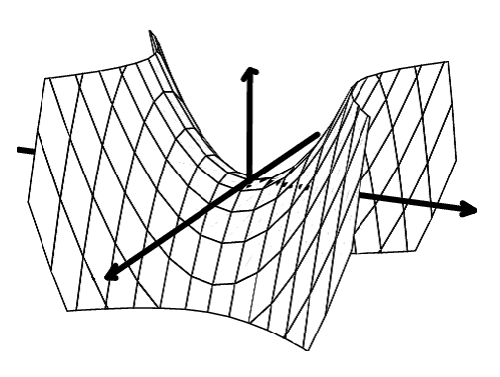
\epsfig{file = sella.eps, width=5cm,clip =}
\end{center}\caption{Gr{\`a}fica de $f(x,y)=x^2-y^2\,.$}\label{sell}
\end{figure}

\vspace{0.3cm}
Estudiant la gr{\`a}fica de la funci{\'o} $ f $ podem veure que $ f (0,0) $ {\'e}s un
m{\`a}xim en la direcci{\'o} de l'eix x, per{\`o} que {\'e}s un m{\'\i}nim en la
direcci{\'o} de l'eix y (quan tallem la superf{\'\i}cie amb plans
paral.lels al pla $ yz $ i $ xz $ respectivament).

\vspace{0.2cm}
Tenim que $f$ {\'e}s diferenciable en tot $\R^2$ i verifica
\[
\begin{cases}
\frac{\partial f}{\partial x}(x,y) = 2x \\
\\
 \frac{\partial f}{\partial y}(x,y) = -2y
\end{cases} \Longrightarrow \begin{cases}
\frac{\partial f}{\partial x}(0,0) = 0 \\
\\
 \frac{\partial f}{\partial y}(0,0) = 0
\end{cases}
\]

Per tant $(0,0) $ {\'e}s un punt cr{\'\i}tic. A m{\'e}s, {\'e}s un punt de sella ja que per tot $r>0$ hi ha punts de la bolla $B((0,0),r)$, tals que:
$$
f(r/2,0)=r^2/4>0\qquad f(0,r/2)=-r^2/4<0
$$


\vspace{0.4cm}
\begin{exemple}
Calcular els m{\`a}xims i m{\'\i}nims de la funci{\'o} $ f (x, y) = x ^ 2 +y ^ 2 $.
\end{exemple}

\solucio
Observam que $ f (x, y) = x ^ 2 +y ^ 2 $ {\'e}s una funci{\'o} diferenciable en
$ \R ^ 2 $, per tant, els extrems de $ f $ s'han de trobar entre
el conjunt de punts cr{\'\i}tics de $ f $.

Calculem els punts cr{\'\i}tics de $ f $ resolent el sistema de
equacions
\[
\begin{cases}
\displaystyle\frac{\partial f}{\partial x}(x,y) = 2x \\
\\
\displaystyle \frac{\partial f}{\partial y}(x,y) = 2y
\end{cases} \Longrightarrow \begin{cases}
\displaystyle\frac{\partial f}{\partial x}(0,0) = 0 \\
\\
\displaystyle \frac{\partial f}{\partial y}(0,0) = 0
\end{cases}
\]
L'{\'u}nic punt cr{\'\i}tic de $ f $ {\'e}s el punt $ (x, y) = (0,0) $ i el seu valor
{\'e}s $ f (0,0) = 0 $. Observem que $ f (x, y) = x ^ 2+y ^ 2 \geq 0 = f (0,0) $ per
tot $ (x, y) \in \R ^ 2 $, per tant en el punt $ (0,0) $ la funci{\'o} $ f $
assoleix el seu m{\'\i}nim. De fet {\'e}s un m{\'\i}nim global. Observau que la
gr{\`a}fica de $ f $ {\'e}s un paraboloide.
\begin{figure} [h!]
\begin{center}
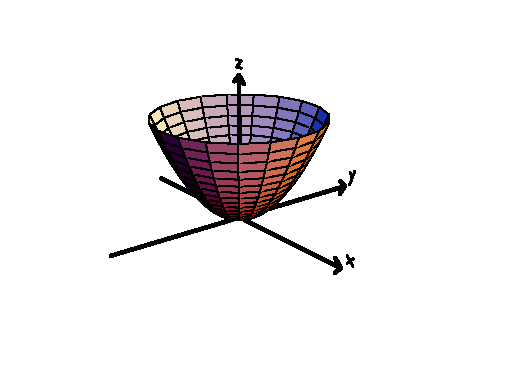
\psfig{file = paraboloide.eps,  width=6.3cm,clip =}
\end{center}\caption{Gr{\`a}fica de $f(x,y)=x^2+y^2\,.$}
\end{figure}



\vspace{0.4cm}
\begin{exemple}
Calcular els m{\`a}xims i m{\'\i}nims de la funci{\'o}
$ f (x, y) = x ^ 2 +y ^2-2x-6y + 14$.
\end{exemple}

\solucio
Observam que igual que abans, $ f $ {\'e}s una funci{\'o} diferenciable
en tot $ \R ^ 2 $, per tant, els extrems de $ f $ s'han de
trobar entre el conjunt de punts cr{\'\i}tics de $ f $.

Calculem els punts cr{\'\i}tics de $ f $ resolent el sistema de
equacions

\[
\begin{cases}
\frac{\partial f}{\partial x}(x,y) = 2x-2 =0\\
\\
 \frac{\partial f}{\partial y}(x,y) = 2y-6=0
\end{cases}
\]

L'{\'u}nic punt cr{\'\i}tic de $ f $ {\'e}s el punt $ (x, y) = (1,3) $ i el seu valor
{\'e}s $ f (1,3) = 4 $. Completant quadrats podem veure que
\[
f (x, y) =  (x-1) ^ 2+ (y-3) ^ 2 +4\geq 4= f (1,3) \qquad \forall
(x, y) \in \R ^ 2.
\]

D'aqu{\'\i} $ f (1,3) = 4 $ {\'e}s un valor m{\'\i}nim de $ f $. De fet en el aquest punt
la funci{\'o} assoleix el seu m{\'\i}nim global.

\vspace{0.4cm}
Per tal d'obtenir condicions suficients per l'exist{\`e}ncia d'extrems relatius definim primer el seg{\"u}ent concepte.

%\vspace{0.4cm}
%\begin{definicio}
%Donada una matriu quadrada d'ordre $n,\ $ $A=(a_{ij})\ \ a_{ij}\in\R$, s'anomena
%\textbf{forma quadr{\`a}tica associada a $A$} a l'funci{\'o}: $\ q_A:\R^n\longrightarrow \R $ definida per:
%$$
%q_A(h)=\sum\limits_{i,j=1}^n\, a_{ij}\,h_ih_j
%$$
%
%o en forma matricial:
%
%$$
%q_A(h)=\left (\begin{matrix}
%   h_1 &
%   h_2 & \ldots & h_n \end{matrix} \right)
%   \left (\begin{matrix}
%   a_{11} &    a_{12} & \ldots & a_{1n}  \\
%
%   a_{21} &    a_{22} & \ldots & a_{2n}\\
%
%    \vdots & \vdots & \ddots & \vdots \\
%
%    a_{n1} &    a_{n2} & \ldots & a_{nn}\end{matrix} \right)
%    \left (\begin{matrix}
%   h_1 \\
%   h_2 \\
%    \vdots\\
%     h_n \end{matrix} \right)
%$$
%\end{definicio}
%
%\vspace{0.4cm}
%\observacions 1.- $q_A(h)$  {\'e}s un polinomi respecte a les variables $h_1,\ldots,h_n$ i per tant una funci{\'o} de classe $\mathcal{C}^\infty(\R^n)$.
%
%2.- Si $\lambda\in\R\,,$ es verifica que $q_A(\lambda\, h)=\lambda^2 q_A(h)$

%\vspace{0.4cm}
%\begin{definicio}
%Direm que la forma quadr{\`a}tica $q_A$ {\'e}s \textbf{definida positiva (negativa)} si
%$$
%q_A(h)>0\qquad (q_A(h)<0)\qquad\qquad \forall h\in\R^n-\{0\}
%$$
%
%Es diu que la forma quadr{\`a}tica es \textbf{semidefinida positiva (negativa)} si
%
%$$
%q_A(h)\geq0\qquad (q_A(h)\leq0)\qquad\qquad \forall h\in\R^n
%$$
%
%Es diu que la forma quadr{\`a}tica es \textbf{indefinida} si existeixen $h_1,h_2\in\R^n$ tals que
%
%$\ q_A(h_1)>0\qquad q_A(h_2)<0\,.$
%\end{definicio}

\vspace{0.4cm}
\begin{definicio}
Sigui $ U \subset \R ^ n $ un obert i $ f :U \subset
\R ^ n \longrightarrow \R $ . Suposem que $f$ t{\'e} totes les derivades de segon ordre en el punt $x _0 \in U $.
Anomenam \textbf{matriu hessiana de $ f $ a $ x_0 $} a la matriu

$$
 Hf(x_0)  = \left (\begin{matrix}
   \displaystyle{\frac{\partial ^ 2 f}{\partial x_1 ^ 2} (x_0)} &
   \displaystyle{\frac{\partial ^ 2 f}{\partial x_2 \partial
x_1} (x_0)} & \ldots & \displaystyle{\frac{\partial ^ 2 f}{\partial
x_n \partial x_1} (x_0)} \\ \\  \displaystyle{\frac{\partial ^ 2 f}{\partial x_1 \partial x_2} (x_0)} &
  \displaystyle{\frac{\partial ^ 2 f}{\partial x_2 ^ 2} (x_0)}
 & \ldots & \displaystyle{\frac{\partial ^ 2 f}{\partial x_n \partial
x_2} (x_0)} \\ \vdots & \vdots & \ddots & \vdots \\  \displaystyle{\frac{\partial ^ 2 f}{\partial x_1 \partial x_n} (x_0)} &
   \displaystyle{\frac{\partial ^ 2 f}{\partial x_2 \partial
   x_n} (x_0)}
 & \ldots & \displaystyle{\frac{\partial ^ 2 f}{\partial x_n ^ 2} (x_0)} \\  \end{matrix} \right) \\
$$
\end{definicio}


%\vspace{0.4cm}
%\begin{definicio}
%Sigui $ U \subset \R ^ n $ un obert i $ f :U \subset
%\R ^ n \longrightarrow \R $ . Suposem que $f$ t{\'e} totes les derivades de segon ordre en el punt $x _0 \in U $. A la forma quadr{\`a}tica associada a la matriu hessiana $Hf(x_0)$, l'anomenam \textbf{hessi{\`a} de $ f $ en  $ x_0$}
%
%\[
%H_{x_0}(f) (h) = \sum_{i, j = 1} ^ n \frac{\partial ^ 2 f}{\partial x_i \partial
%x_j} (x_0) \, h_i  h_j \qquad h = (h_1, h_2, \ldots, h_n) \in \ R ^ n.
%\]
%\end{definicio}


\vspace{0.4cm}
Ara ja podem establir diversos criteris per tal de
classificar els punts cr{\'\i}tics d'una funci{\'o} $ f $.

\vspace{0.4cm}
\begin{teorema}\label{valors propis}
Sigui $ U \subset \R ^ n $ un obert i $ f \,: \, U \subset
\R ^ n \longrightarrow \R $ una funci{\'o} que admet totes les derivades parcials segones i s{\'o}n cont{\'\i}nues. Sigui $ x_0 \in
U $ un punt cr{\'\i}tic de $ f $. Sigui $\  Hf(x_0)\ $ la seva matriu hessiana. Llavors:
\begin{itemize}
\item [a)]  $f$ t{\'e} un m{\'\i}nim relatiu en $ x_0 $ si, i nom{\'e}s si, tots els valors propis de $Hf(x_0)$ s{\'o}n positius.
\item [b)]  $f$ t{\'e} un m{\`a}xim relatiu en $ x_0 $ si, i nom{\'e}s si, tots els valors propis de $Hf(x_0)$ s{\'o}n negatius.
\item [c)]  $f$ t{\'e} un punt de sella en $ x_0 $ si, i nom{\'e}s si, $Hf(x_0)$ t{\'e} valors propis positius i negatius.
\end{itemize}
\end{teorema}


\vspace{0.4cm}
\begin{teorema}\label{clasificacio}
Sigui $ U \subset \R ^ n $ un obert i $ f \,: \, U \subset
\R ^ n \longrightarrow \R $ una funci{\'o} que admet totes les derivades parcials segones i s{\'o}n cont{\'\i}nues. Sigui $ x_0 \in
U $ un punt cr{\'\i}tic de $ f $.  Sigui $\  Hf(x_0)\ $ la seva matriu hessiana, i sigui  $\Delta_k$ el seu menor principal d'ordre $k$. Llavors:
\begin{itemize}
\item [a)] Si $\ \Delta_k>0 \ \ k=1,\ldots, n\,, $ llavors $f$ t{\'e} un m{\'\i}nim relatiu en $ x_0 $.
\item [b)] Si $\ (-1)^k\Delta_k>0 \ \ k=1,\ldots, n\,, $ llavors $ f $ t{\'e} un m{\`a}xim relatiu en $ x_0 $.
\end{itemize}
\end{teorema}

\vspace{0.4cm}
\observacio Els dos resultats anteriors no cobreixen totes les possibilitats. En els casos no contemplats, hi ha que fer altres estudis per poder decidir quin tipus de punt cr{\'\i}tic tenim.

\vspace{0.4cm}
En el cas  $ n = $ 2 podem escriure el seg{\"u}ent resultat.

\vspace{0.4cm}
\begin{teorema}
Sigui $ U \subset \R ^ 2 $ un obert i $ f \,: \, U \subset
\R ^ 2 \longrightarrow \R $ una funci{\'o} que admet totes les derivades parcials segones i s{\'o}n cont{\'\i}nues. Sigui
$ (a, b) \in U $ un punt cr{\'\i}tic de $ f $. Considerem
\[
Hf (a, b) =
  \left (\begin{matrix}
    \displaystyle\frac{\partial ^ 2 f}{\partial x_1 ^ 2} (a, b) & \displaystyle\frac{\partial ^ 2 f}{\partial x_2 \partial
x_1} (a, b) \\
\\
\displaystyle\frac{\partial ^ 2 f}{\partial x_1\partial x_2}    (a, b) &  \displaystyle\frac{\partial ^ 2 f}{\partial x_2 ^ 2}(a, b)
  \end{matrix} \right)
= \left (\begin{matrix}
    A & B \\    B & C
  \end{matrix} \right)
\quad \mbox{i sigui} \quad \Delta = AC-B ^ 2.
\]
\begin{itemize}
\item [a)] Si $ \Delta> 0 $ i $ A> 0 $, llavors $ f $ t{\'e}  un
m{\'\i}nim local en $ (a, b) $.
\item [b)] Si $ \Delta> 0 $ i $ A <0 $, llavors $ f $ t{\'e} un
m{\`a}xim local en $ (a, b) $.
\item [c)] Si $ \Delta <0 $, llavors $ f $ t{\'e} un
punt de sella en $ (a, b) $.
\item [d)] Si $ \Delta = 0 $,  no podem dir res sobre el punt $ (a, b) $.
\end{itemize}
\end{teorema}


\vspace{0.4cm}
\begin{exemple}
Trobau els extrems de la funci{\'o} $\ f (x, y) = x^4 + y^4-4xy +1 $.
\end{exemple}

\solucio
Trobem  primer els punts cr{\'\i}tics de $ f $
resolent el sistema d'equacions

\[
\begin{cases}
\displaystyle\frac{\partial f}{\partial x} = 0 \\
 \\
 \displaystyle\frac{\partial f}{\partial y} = 0
\end{cases} \Longrightarrow \begin{cases}
4x ^ 3 - 4y = 0 \\
\\
4y ^ 3-4x = 0
\end{cases} \Longrightarrow \begin{cases}
x ^ 3 - y = 0 \\
\\
y ^ 3 - x = 0.
\end{cases}
\]
Per resoldre el sistema d'equacions prenem $\ y = x ^ 3 $ de la
primera equaci{\'o} i la substitu{\"\i}m en la segona, obtenint
\begin{align*}
x ^ 9-x & = x (x ^ 8 -1) = x (x ^ 4 -1) (x ^ 4 +1) = x (x ^ 2-1) (x ^ 2 +1) (x ^ 4 +1) \\& = x (x-1) (x +1) (x ^ 2 +1) (x ^ 4 +1)
\end{align*}

\noindent aix{\'\i}, les solucions s{\'o}n $ x = 0 $, $ x = 1 $ i $ x =- 1 $. Els
punts cr{\'\i}tics s{\'o}n $ (0,0) $, $ (1,1) $ i $ (-1, -1) $. Per
classificar-lo utilitzem el teorema anterior. Calculem primer
la matriu hessiana.

\[
Hf (x, y) =
  \left (\begin{matrix}
    12x ^ 2 & -4 \\    -4 & 12y ^ 2
  \end{matrix}\right), \qquad \Delta = 144 x ^ 2 y ^ 2 -16 \quad \mbox{i} \quad
  A = 12x ^ 2
\]

Considerant cada un dels punts cr{\'\i}tics obtinguts tenim
que:
\begin{itemize}
\item [] $ (0,0)\ $: $\ \Delta (0,0) =- 16 <0 $, llavors en $ (0,0) $ la
funci{\'o} t{\'e} un punt de sella.
\item [] $ (1,1)\ $: $\ \Delta (1,1) = 144-16> 0 $ i $ A = 12> 0 $,
llavors en $ (1,1) $ la funci{\'o} assoleix un m{\'\i}nim local.
\item [] $ (-1, -1)\ $: $\ \Delta (-1, -1) = 144-16> 0 $ i $ A = 12> 0 $,
llavors  la funci{\'o} t{\'e} en $ (-1, -1) $ un m{\'\i}nim local.
\end{itemize}


%\vspace{0.4cm}
%\begin{exemple}
%Trobau la dist{\`a}ncia m{\'e}s curta del punt $ (1,0,-2) $ al pla
%$ x +2 y + z = 4 $.
%\end{exemple}
%
%\solucio
%La dist{\`a}ncia d'un punt $ (x, y, z) $ al punt $ (1,0, -2) $ ve donada
%per
%\[
%d = \sqrt{(x-1) ^ 2 + y ^ 2 + (z +2) ^ 2},
%\]
%per{\`o} com el punt $ (x, y, z) $ ha d'estar en el pla
%$ x +2 y + z = 4 $, llavors $ z = 4-x-2y $ i per tant la funci{\'o} a minimitzar
%{\'e}s
%
%\[
%d (x, y) = \sqrt{(x-1) ^ 2 + y ^ 2 + (4-x-2y +2) ^ 2} = \sqrt{(x-1) ^ 2 + y ^ 2 +
%(6-x-2y) ^ 2}.
%\]
%
%Podem trobar la dist{\`a}ncia m{\'\i}nima demanada minimitzant $ d $ o
%b{\'e} $ d ^ 2 $. Aix{\'\i}, minimitzarem la funci{\'o}
%
%\[
%f (x, y) = (x-1) ^ 2 + y ^ 2 + (6-x-2y) ^ 2= 2 x^2 + 4 x y + 5 y^2- 14 x- 24 y+37   .
%\]
%
%Cerquem els punts cr{\'\i}tics de $ f $:
%
%\begin{align*}
%\frac{\partial f}{\partial x} & = 4x
%+4 y-14 = 0 \\
%&\\ \frac{\partial f}{\partial y} & =  4x +10 y-24 = 0
%\end{align*}
%
%L'{\'u}nic punt cr{\'\i}tic {\'e}s $ (11 / 6,5 / 3) $. Com $\ f_{xx} = 4 $,
%$ f_{xy} = 4\ $ i $\  f_{yy} = 10 $
%
%\[
%\Delta = 4 \cdot 10 -4 ^ 2 = 40-16 = 24> 0, \quad \mbox{i} \quad
%A = f_{xx} = 4> 0
%\]
%
%En definitiva, en el punt $ (11 / 6,5 / 3) $ la funci{\'o} assoleix un m{\'\i}nim local i la dist{\`a}ncia m{\'\i}nima ve donada per
%\[
%d = \sqrt{f (11 / 6,5 / 3)} = \frac{5 \sqrt{6}}{6}.
%\]


\vspace{0.4cm}
\begin{exemple}
Trobau  els m{\`a}xims i m{\'\i}nims relatius de la
funci{\'o}
\[
f (x, y) = x ^ 2 e ^{-x ^ 2-y ^ 2}
\]
\end{exemple}

\solucio
Per calcular els punts cr{\'\i}tics de $ f $ calculem primer les seves
derivades parcials

$$
\frac{\partial f}{\partial x} (x, y)  =  (2x-2x ^ 3) e ^{-x ^ 2-y ^ 2}
\qquad\qquad
\frac{\partial f}{\partial y} (x, y)  =    -2x ^ 2y e ^{-x ^ 2-y ^ 2}
$$

Un punt $ (x, y) $ ser{\`a} un extrem relatiu de $ f $ si

\[
\left.
\begin{array}{r}
  (2x-2x ^ 3) e ^{-x ^ 2-y ^ 2} = 0 \\   -2x ^ 2ye ^{-x ^ 2-y ^ 2} = 0
\end{array}
\right \} \, \; \Longrightarrow \, \; \left.
\begin{array}{r}
  x (1-x ^ 2) = 0 \\   x ^ 2y = 0
\end{array}
\right \}
\]

De la primera equaci{\'o} obtenim $ x = 0\ $ o $\ x = \pm 1 $.

\begin{itemize}
\item [] Si $ x = 0 $, de la segona equaci{\'o} $ y $ pot prendre qualsevol
valor. Obtenim, per tant, els punts $ (0, y)\,,\ \ y \in \R $.
\item [] Si $ x = \pm 1 $, de la segona equaci{\'o} $ y = 0 $. Obtenim, per tant,
els punts $ (1,0) $, $ (-1,0) $.
\end{itemize}

Per classificar els punts cr{\'\i}tics calculem en primer lloc les
derivades parcials de segon ordre de $ f $.
\begin{align*}
  \frac{\partial ^ 2 f}{\partial x ^ 2} (x, y) & = (2-10x ^ 2 + 4x ^ 4) e ^{-x ^ 2-y ^ 2} \\
  \frac{\partial ^ 2 f}{\partial x \partial y} (x, y) & = 4y (x ^ 3-x) e ^{-x ^ 2-y ^ 2} \\
  \frac{\partial ^ 2 f}{\partial y ^ 2} (x, y) & = 2x ^ 2 e ^{-x ^ 2-y ^ 2}
   (2y ^ 2-1)
\end{align*}

Aix{\'\i}, considerant cada un dels punts cr{\'\i}tics i avaluant les
derivades parcials de segon ordre en cada un d'ells
obtenim el seg{\"u}ent.

\begin{itemize}
\item [] Punt $ (0, y) $:

\[
\frac{\partial ^ 2 f}{\partial x ^ 2} (0, y) = 2e ^{-y ^ 2}, \, \quad
\frac{\partial ^ 2 f}{\partial x \partial y} (0, y) = 0, \, \quad
\frac{\partial ^ 2 f}{\partial y ^ 2} (0, y) = 0.
\]
Aix{\'\i}, com
\[
\left |
\begin{matrix}
  2e ^{-y ^ 2} & 0 \\  0 & 0
\end{matrix}
\right | = 0
\]

el criteri no decideix. Per{\`o} com $ f (0, y) = 0 $, i en qualsevol
entorn del punt $ (0, y) $, si $ (u, v) $ {\'e}s un punt d'aquest entorn
es t{\'e} que $\ f (u, v) = u ^ 2e ^{-u ^ 2-v ^ 2} \geq 0 = f (0, y) $, tenim que
en els punts de la forma $ (0, y) $ la funci{\'o} $ f $ assoleix m{\'\i}nims
relatius. A m{\'e}s el seu valor {\'e}s $\ f (0, y) = 0 $.

\item [] Punts $ (1,0), (-1,0) $:

\[
\frac{\partial ^ 2 f}{\partial x ^ 2} (\pm 1,0) =- 4 e ^{-1}, \, \quad
\frac{\partial ^ 2 f}{\partial x \partial y} (\pm 1,0) = 0, \, \quad
\frac{\partial ^ 2 f}{\partial y ^ 2} (\pm 1,0) =- 2 e ^{-1}.
\]

Aix{\'\i}, com
\[
\left |
\begin{matrix}
  -4 e ^{-1} & 0 \\
   0 &-2 e ^{-1}
\end{matrix}
\right | = 8e ^{-2} >0, \, \quad \mbox{i} \, \quad \frac{\partial ^ 2
f}{\partial x ^ 2} (\pm 1,0) =- 4 e ^{-1} <0
\]

tenim que en els punts $\ (1,0), (-1,0)\ $ la funci{\'o} $ f $ arriba a un m{\`a}xim
relatiu. La funci{\'o} val $\ f(1,0)=f(-1,0)=1/e\,.$
\end{itemize}

\subsubsection{Extrems absoluts}

Ja hem vist en el tema de continu{\"\i}tat el Teorema de Weierstrass que ens diu que si $K\subset
\R ^ n$ {\'e}s un conjunt compacte i si $\ f :K  \longrightarrow \R $,    {\'e}s
una funci{\'o} cont{\'\i}nua en $ K $, llavors $ f $ t{\'e} un m{\`a}xim i un m{\'\i}nim absoluts en $ K$.
Ara b{\'e}, pot passar que s'agafin en un punt interior de $K$ o en la frontera de $K$.

Si $ f $ {\'e}s
diferenciable a l'interior de $ K $, llavors si aquests extrems es troben en l'interior de $K$,
 es donaran en punts cr{\'\i}tics de $ f $.

Aix{\'\i}, per calcular els extrems absoluts de $ f $, si $ f $ {\'e}s
cont{\'\i}nua en $ K $ i diferenciable a l'interior de $ K $, hem de fer el seg{\"u}ent:
\begin{itemize}
\item [1)] Trobar els punts cr{\'\i}tics de
$ f $ en l'interior de $ K $. Despr{\'e}s avaluar $ f $ en aquests punts.
\item [2)] Trobar els extrems de $ f $ a la frontera de $ K $.
\item [3)] Comparar els valors obtinguts en 1) i 2) per
determinar els extrems absoluts.
\end{itemize}

\vspace{0.4cm}
\begin{exemple}\label{extr abs1}
Trobau els extrems absoluts de la funci{\'o} $ f (x, y) = x ^ 2-2 x y +2y $
en el rectangle $\ C = \{(x, y) \in \R ^ 2 \,: \, 0 \leq x \leq 3, \, 0 \leq y
\leq 2 \} $.
\end{exemple}

\solucio
Com $ f $ {\'e}s un polinomi {\'e}s una funci{\'o} cont{\'\i}nua i $ C $ {\'e}s un compacte, podem afirmar que $f$ t{\'e} extrems absoluts en $C$.

Calculem primer el punts cr{\'\i}tics de $ f $ a l'interior de
$ C $.
\[
  \begin{cases}
    \displaystyle\frac{\partial f}{\partial x} = 2x-2y = 0 \\
    \\
       \displaystyle\frac{\partial f}{\partial y} =- 2x +2 = 0
  \end{cases}
\]

llavors l'{\'u}nic punt cr{\'\i}tic en l'interior de $ C $ {\'e}s el punt
$ (1,1) $. Ara com
\[
\Delta = \frac{\partial ^ 2 f}{\partial x ^ 2} \frac{\partial ^ 2
f}{\partial y ^ 2} - \left (\frac{\partial ^ 2 f}{\partial x \partial y}
\right) ^ 2 = 2\cdot 0 - (-2) ^ 2 = -4 <0
\]

tenim que en el punt $ (1,1) $ la funci{\'o} $ f $ assoleix un punt de
sella.

Estudiem ara que passa a la frontera.
\begin{itemize}
\item[$\ast$] $ x = 3: \quad  f (3, y) =  9-4y\,,\quad 0 \leq
y \leq 2\,. $ Ja que $\ f (3, y)\ $ {\'e}s una funci{\'o} decreixent en $ y $ aix{\'\i}, el
m{\`a}xim s'assoleix en $\ y = 0\ $ i el m{\'\i}nim a $\ y = 2\ $ i valen
$\ f (3,0) = 9 \quad  f (3,2) = 1$.

\item[$\ast$] $ x = 0: \quad  f (0, y) = 2y \,,\quad 0 \leq
y \leq 2\,. $ Ja que $\ f (0, y)\ $ {\'e}s una funci{\'o} creixent en $ y $ aix{\'\i}, el
m{\`a}xim s'assoleix a $\ y = 2\ $ i el m{\'\i}nim a $\ y = 0\ $ i valen
$\ f (0,2) = 4 \quad \ f (0,0) = 0.$

\item[$\ast$] $ y = 2: \quad  f (x, 2) = (x-2) ^ 2\,,\quad 0 \leq
x \leq 3\,. $  Com $ f '(x) = 2 (x-2) $, llavors $ x = 2 $ {\'e}s
el punt on $ f (x, 2) $ t{\'e} el seu m{\'\i}nim (ja que $ f''(x) = 2> 0 $) i val $\ f (2,2) = 0\,. $
El m{\`a}xim ho aconsegueix en el punt $ x = 0 $ ja que $\  f (0,2) = 4\quad f(3,2)=1.$

\item[$\ast$] $ y = 0: \quad  f (x, 0) = x ^ 2 \,,\quad 0 \leq
x \leq $ 3, que {\'e}s una funci{\'o} creixent en l'interval $ [0,3] $.
Aix{\'\i}, el m{\`a}xim l'assoleix en el punt $\ x = 3\ $ i el m{\'\i}nim en el
punt $\ x = 0\ $ i valen $\ f (3,0) = 9 \quad f (0,0) = 0$.
\end{itemize}

Comparant entre si els m{\`a}xims i els m{\'\i}nims, tenim que el
m{\`a}xim absolut s'assoleix en el punt $ (3,0) $ i el seu valor {\'e}s
$ f (3,0) = 9 $, i el m{\'\i}nim absolut s'assoleix en els punts $ (0,0) $
i $ (2,2) $ i el seu valor {\'e}s $ f (0,0) = f (2,2) = 0 $.


\vspace{0.4cm}
\begin{exemple}\label{extr abs2}
Trobau els extrems absoluts de la funci{\'o} $ f (x, y) = x ^ 2+y^2- x -y +1 $
en la regi{\'o} $\ K=\{(x,y)\in\R^2 \ : \ x^2+y^2\leq 1 \}$.
\end{exemple}

\solucio
Com $ f $ {\'e}s un polinomi {\'e}s una funci{\'o} cont{\'\i}nua i $ K $ {\'e}s un compacte, podem afirmar que $f$ t{\'e} extrems absoluts en $K$.

Calculem primer el punts cr{\'\i}tics de $ f $ a l'interior de
$ K $.
\[
  \begin{cases}
    \displaystyle\frac{\partial f}{\partial x} = 2x-1 = 0 \\
    \\
       \displaystyle\frac{\partial f}{\partial y} =2y-1 = 0
  \end{cases}
\]

llavors l'{\'u}nic punt cr{\'\i}tic en l'interior de $ K $ {\'e}s el punt
$ (1/2,1/2) $. Ara com
\[
\Delta = \frac{\partial ^ 2 f}{\partial x ^ 2} \frac{\partial ^ 2
f}{\partial y ^ 2} - \left (\frac{\partial ^ 2 f}{\partial x \partial y}
\right) ^ 2 = 2\cdot 2 - (0) ^ 2 = 4 >0\quad\mbox{i} \quad \frac{\partial ^ 2 f}{\partial x ^ 2}(1/2,1/2)>0
\]

tenim que en el punt $ (1/2,1/2) $ la funci{\'o} $ f $ assoleix un m{\'\i}nim local i val $\ f(1/2,1/2)=1/2 $.

Estudiem ara que passa a la frontera de $K$. La podem expressar com
$$\ \partial K=\{(\cos \theta,\sin\theta)\ :\ \theta\in[0,2\pi]\}\ $$

llavors $f$ sobre la frontera ve donada per la funci{\'o}

$$
g(\theta)=2-\cos \theta-\sin\theta
$$

D'on
$$
g'(\theta)=\sin \theta-\cos\theta\,,\qquad g''(\theta)=\cos \theta+\sin\theta
$$

Per tant
$$
g'(\theta)=0\Leftrightarrow \sin \theta=\cos\theta\Rightarrow \theta\in\{\pi/4 ,5\pi/4 \}
$$

 i ja que $\ g''(\pi/4)=\sqrt{2}>0\,,\qquad g''(5\pi/4)=-\sqrt{2}<0\ $ tenim que $g$ t{\'e} un m{\'\i}nim en $\ \theta=\pi/4\ $ que correspon al punt $\ (\sqrt{2}/2,\sqrt{2}/2)\ $ i un m{\`a}xim en $\ \theta=5\pi/4\ $ que correspon al punt $\ (-\sqrt{2}/2,-\sqrt{2}/2)\ $.

 Avaluant la funci{\'o} en aquests punts podrem decidir els extrems absoluts:

 $f(\sqrt{2}/2,\sqrt{2}/2)=2-\sqrt{2}\approx 0.58\qquad f(-\sqrt{2}/2,-\sqrt{2}/2)=2+\sqrt{2}\approx 3.41$.

 En definitiva, en $\ (1/2,1/2)\ $ tenim un m{\'\i}nim absolut de $f$ i val $\ 1/2\,,$ i en $\ (-\sqrt{2}/2,-\sqrt{2}/2)\ $ tenim un m{\`a}xim absolut de $f$ i val $\ 2+\sqrt{2}\,.$



\end{document}









